\documentclass[12pt]{article}
\usepackage{fontspec}

\setmainfont{Times New Roman} % Times New Roman, Arial, Calibri

\usepackage{setspace}
\setstretch{1.15}

\usepackage{pdflscape}

\usepackage{graphicx}
\usepackage{float}
\usepackage{placeins}
%\usepackage[backend=biber, style=authoryear]{biblatex}
\usepackage[backend=biber, style=numeric]{biblatex}
\addbibresource{references.bib}

\usepackage{geometry}
\geometry{top=2.5cm, bottom=2.5cm, left=2.5cm, right=2.5cm}

\usepackage{pdfpages}

\usepackage{listings}
\usepackage{xcolor}
% Define colors
\definecolor{codegreen}{rgb}{0,0.6,0}
\definecolor{codegray}{rgb}{0.5,0.5,0.5}
\definecolor{codepurple}{rgb}{0.58,0,0.82}
\definecolor{backcolour}{rgb}{0.95,0.95,0.92}

% Setup the listings package
\lstdefinestyle{mystyle}{
    backgroundcolor=\color{backcolour},
    commentstyle=\color{codegreen},
    keywordstyle=\color{magenta},
    numberstyle=\tiny\color{codegray},
    stringstyle=\color{codepurple},
    basicstyle=\ttfamily\footnotesize,
    breakatwhitespace=false,
    breaklines=true,
    captionpos=b,
    keepspaces=true,
    numbers=left,
    numbersep=5pt,
    showspaces=false,
    showstringspaces=false,
    showtabs=false,
    tabsize=2
}

\lstset{style=mystyle}

\usepackage{amsmath} % For mathematical features

\renewcommand{\theequation}{\thesection.\arabic{equation}}
\renewcommand{\thefigure}{\thesection.\arabic{figure}}

\usepackage{chngcntr}
\counterwithin{figure}{section}
\counterwithin{equation}{section}

\title{Identifying Dynamic Systems with Probabilistic Numerics}
\author{Harvey Walton}
\date{\today}

%Repeated Text
\newcommand{\ndiFigCaption}[1]{The rectangle method for finding the #1 bound of the integral of the standard Gaussian (normal) distribution between -2 and 1.}

\hyphenpenalty=700
\exhyphenpenalty=700

\begin{document}
    \pagenumbering{roman}

    \thispagestyle{empty}
    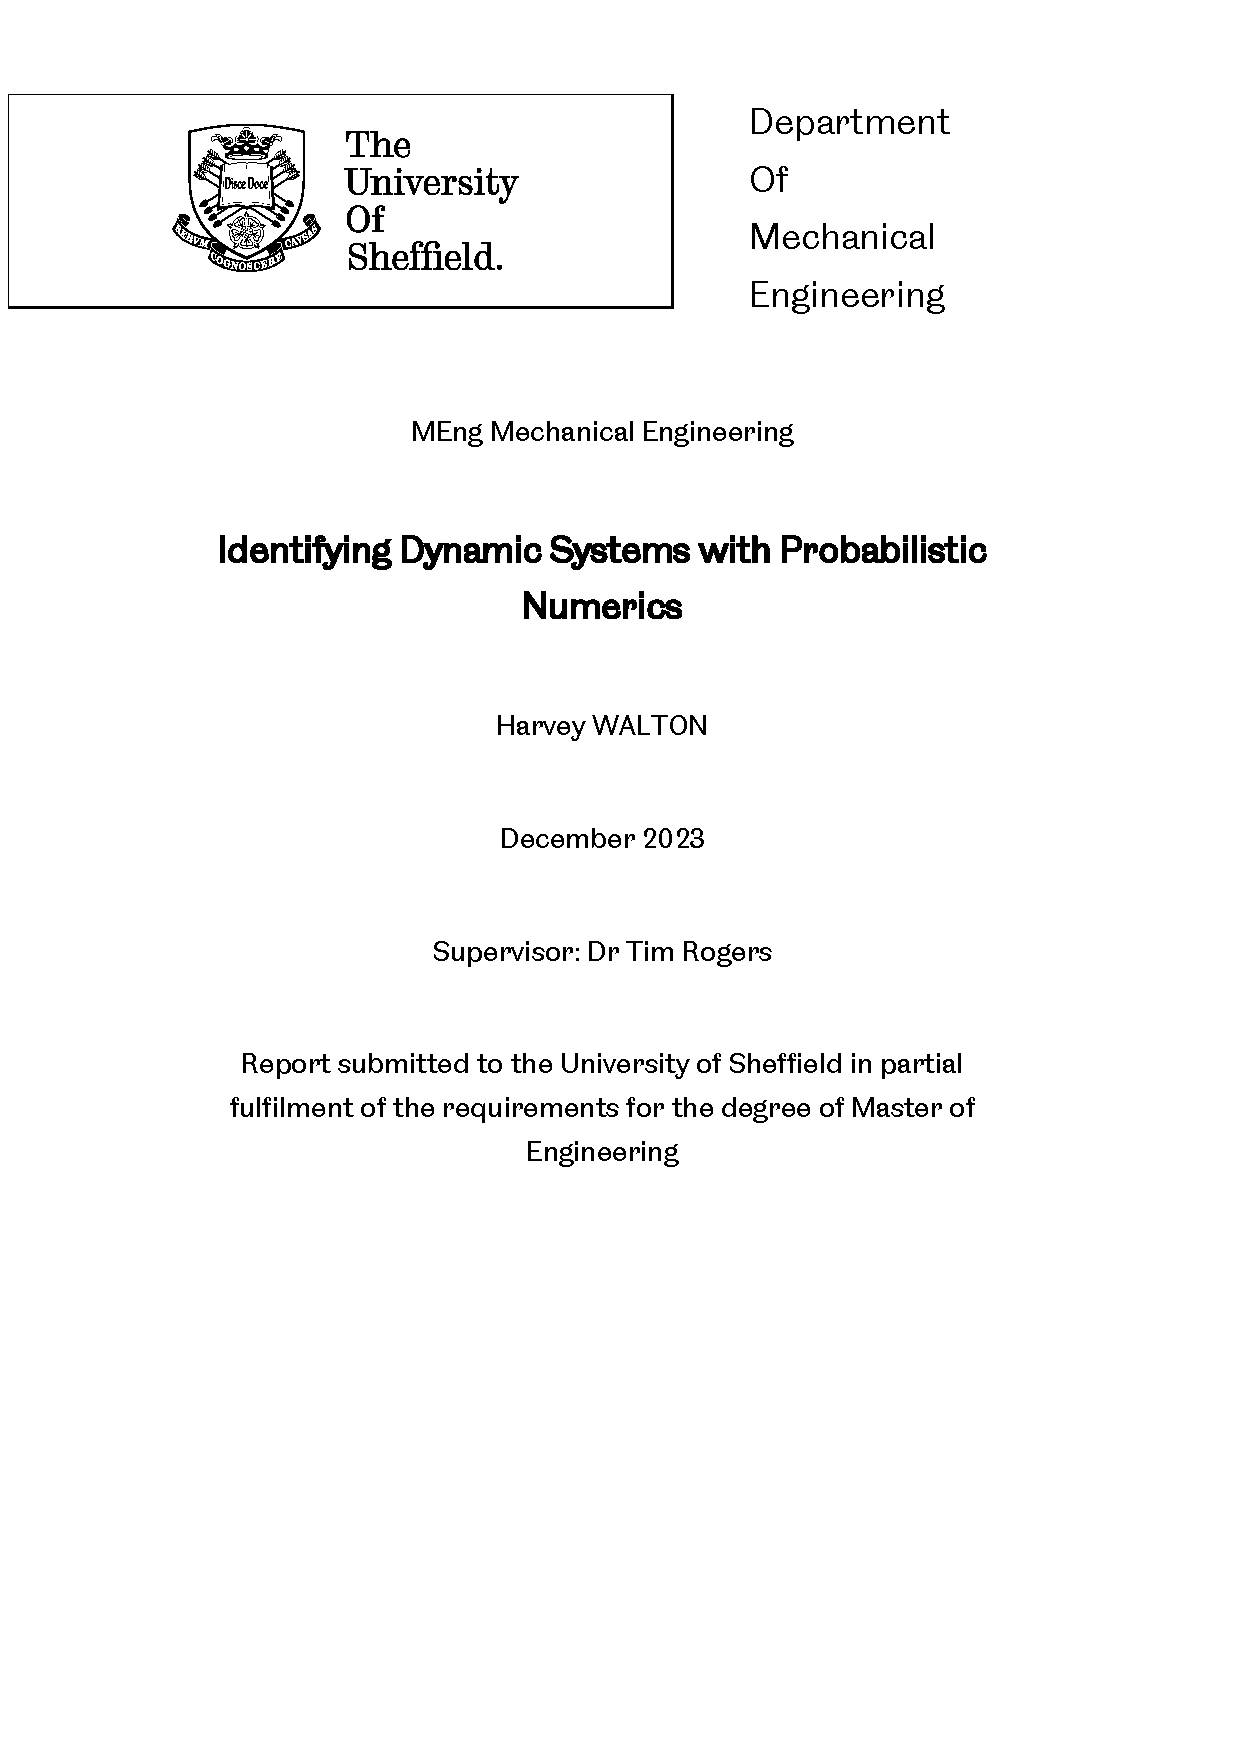
\includepdf[pages=1, frame, scale=1.09, pagecommand={}, offset=0 -35]{figures/titlepage.pdf}


    \tableofcontents
    \newpage

    \pagenumbering{arabic}

    \section{Background and Understanding of the Problem}


    Problems in engineering are usually described using a framework of continuous mathematical functions.
    This means that their output has no jumps or gaps in values, and they can be evaluated using input values that are on a sliding scale of a continuous input domain.
    For example, time in the real world is on a continuous sliding scale, which means that any interval in time can always be subdivided into a smaller interval.
    Continuous functions in turn can often be manipulated analytically using mathematics.
    For example, if the velocity of a particle is given as a continuous function of time, a continuous acceleration function can be derived from the velocity analytically through a mathematical process called differentiation.

    \subsection{The Limits of the analytical approach}

    However, there are many situations where this analytical approach is unsuitable.
    Classically, numerical methods will be used to approximate the true solution.

    \subsubsection{Intractable Complexity}

    The first reason for this is that the analytical approach may be too complex for anyone to solve.
    A good example of this is the Gaussian (normal) distribution (Equation~\ref{eq:norm}). %\cite{NIST2023}

    \begin{equation}
        f(x) = \frac{1}{\sigma\sqrt{2\pi}} \exp\left(-\frac{(x - \mu)^2}{2\sigma^2}\right)\label{eq:norm}
    \end{equation}

    This definite integral of this is often needed in order to find cumulative probabilities (i.e., the chances of a continuous random variable being in a range defined by two values).
    This process can be visualised as finding the area underneath the curve between 2 input values (Figure~\ref{fig:ndi_}).

    \begin{figure}[htbp]
        \centering
        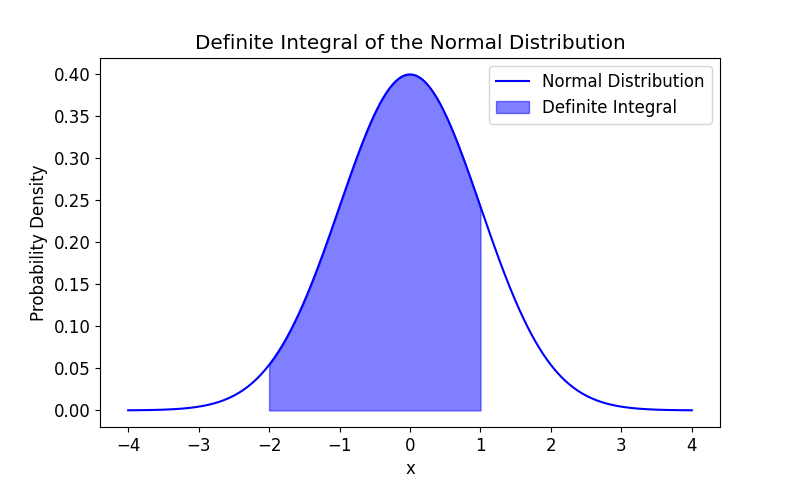
\includegraphics[width=0.8\linewidth]{figures/ndi/ndi_}
        \caption{A definite integral between -2 and 1 of the standard Gaussian (normal) distribution. This is used to find cululative probabilities.}
        \label{fig:ndi_}
    \end{figure}

    In this case, a numerical method is typically used instead such as the Rectangle Method, which uses the Riemann integral definition.
    This states that an integral can be approximated by summing the area of many adjacent rectangles between the function and the axis~\cite{NumericalAnalysis2023}, as shown in Figure~\ref{fig:ndi-num_} and Figure~\ref{fig:ndi-num2_}.

    \FloatBarrier

    \begin{figure}[htbp]
        \centering
        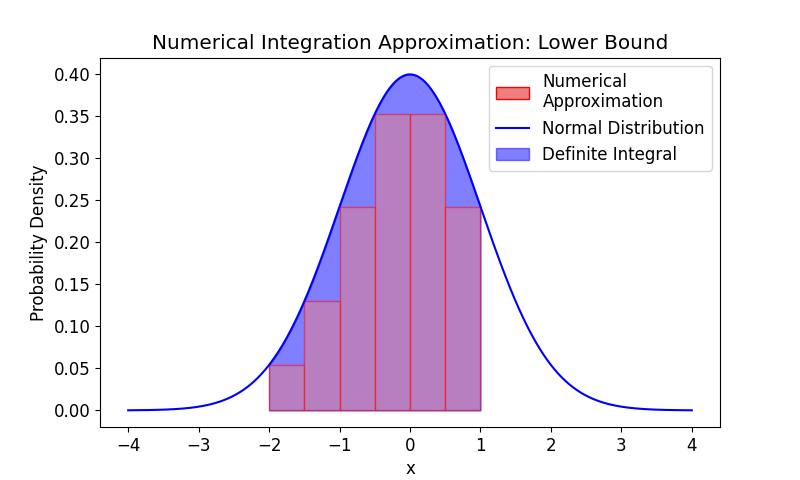
\includegraphics[width=0.8\linewidth]{figures/ndi-num/ndi-num_}
        \caption{\ndiFigCaption{lower}}
        \label{fig:ndi-num_}
    \end{figure}

    \FloatBarrier

    \begin{figure}[htbp]
        \centering
        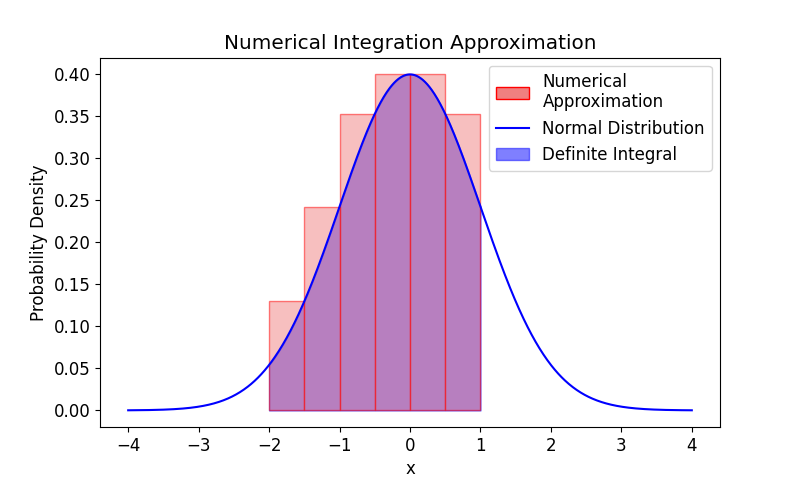
\includegraphics[width=0.8\linewidth]{figures/ndi-num2/ndi-num2_}
        \caption{\ndiFigCaption{upper}}
        \label{fig:ndi-num2_}
    \end{figure}
    As the width of the rectangles approaches zero, the approximation increasingly converges to the exact value of the integral.
    This can never happen in practice, however, because it would require infinite computational work.
    However, we can get good
    As you can see, there are two ways to draw the rectangles.
    In the first method, the top corner of the two that touches the curve is chosen such that the top edge is below the curve.
    This provides an underestimate, which we can use as a lower bound to the true value of the integral.
    Whereas in the second method, the top corner of the two that touches the curve is chosen such that the top edge is above the curve.
    This provides an overestimate, which we can use as an upper bound to the true value of the integral.
    Classically, the quality of this numerical method is computed using the ``error bounds`` ie range between these upper and lower values.

    \subsubsection{Data Sampling}
    The second situation where the analytical approach is unsuitable is when working with real world data.
    Here, the real world continuous data streams of the variables you are measuring must be sampled at a number of individual (or ``discrete``) points in time.
    A simple example of this is how a video camera discretises the continuous events of the world into individual frames (or ``samples``) that can be replayed back-to-back to recreate an approximation of the events.
    As the frame rate increases, the events are captured in more detail, but the amount of information required to store the approximation tends to infinity and the length of time between frames tends to zero.
    This discrete data is unsuitable for analytical mathematical methods that rely on the data being continuous cannot be implemented.
    Again, there are numerical methods that are commonly used to approximate this instead.
    For example, differentiation is the process of finding the gradient of a continuous function at any location along the curve.
    For a discrete function, the gradient at any point is undefined because you cannot have a tangent of a point.
    However, it is possible to approximate the gradient of the underlying continuous function from which the data was sampled using a numerical method, such as the Forward Difference Method.
    This simply approximates the underlying continuous function as a straight line joining each point.
    Therefore, the gradient at a point is calculated as the slope between that point and a point at a distance h ahead.

    Data from experimentally measured signals also contains noise from many sources.
    For example, accelerometer data may be mixed with noise from random vibrations caused by the surroundings (people walking, movement of traffic nearby etc.), as well as simply the imprecision of the measuring device, which may be significant in proportion to the signal.
    Again, the uncertainty caused by this noise is classically defined by error bounds (i.e., giving a measurement with a tolerance such as $3.5 \pm 0.7 ms^{-2}$)

    \subsection{An alternative to numerical methods}

    However, this paper investigates an alternative modelling and analysis process that allows the continuous signal to be reconstructed from discrete sample data.
    Since this reconstruction is in closed form, it can still be manipulated using analytical techniques.
    The alternative process uses a type of machine learning model called a Gaussian Process, which uses discrete data points to create a continuous function that interpolates between these points.
    This model is special because it generates outputs probabilistically, meaning that the output for a given input (point) is not a single point.
    Instead, it is a Gaussian probability distribution defined by a mean and standard deviation, which are both a continuous closed form function of the input (time).
    Therefore, not only does this technique allow for experimentally collected data to be manipulated using analytical mathematical techniques, it also captures the noise in a new way - by modeling it with uncertainty (i.e., a probability distribution) instead of error bounds (as is used classically).
    The improvements in the robustness of manipulations of noisy data due to this new way of modelling uncertainty are investigated in the context of a technique called the Fourier transform as defined in Equation~\ref{eq:ft} where \( \omega \) is the angular frequency.

    \begin{equation}
        F(\omega) = \int_{-\infty}^{\infty} f(t) e^{-i \omega t} \, dt\label{eq:ft}
    \end{equation}


    This is an extremely powerful analytical technique that is used widely in engineering contexts.
    It is a transformation that takes a function in the time domain, and produces a function in the frequency domain.
    It has a mathematical definition that takes function that has a continuous time domain, and transforms it into a function that has a continuous frequency domain.
    Therefore, the gaussian process will be used to preprocess the discrete sample data into a continuous closed from, from which the Fourier transform can be applied.
    The efficiency of this approach will be evaluated in comparison to the discrete version of this transformation known as the Fast Fourier Transform (FFT) algorithm.
    This is classically used when working with sampled data, but has numerous drawbacks when compared to the continuous Fourier transform.

    \subsection{Drawbacks of the Fast Fourier Transform Algorithm}
    Although discovering a fast way to compute the discrete Fourier Transform revolutionised many engineering disciplines such as structural health monitoring, image compression, signal processing, and control theory\cite{Byjus2023}, its implementation has a number of challenges that have to be carefully handled.
    The first is that the FFT assumes the signal is periodic, which can lead to a phenomenon called spectral leakage if the signal is not an exact multiple of the chosen window\cite{MathStackExchange2023}.
    This can cause sharp resonance peaks to be smoothed out in the output because energy that should be concentrated at a peak frequency is spread across a range of frequencies nearby.

    Secondly, the FFT can be highly sensitive to noise in the data, which can create fluctuations in the frequency spectrum, masking the true underlying frequencies\cite{MathStackExchange2023}.



    \subsection{Implications of the Findings}

    \subsubsection{Implications in the Context of the Fourier Transform}

    Therefore, whether this new proposed method for computing Fourier transforms can do so with less pronounced spectral leakage issues and more noise resilience will be investigated.
    The comparison of the two approaches is done in the context of modal analysis of a Multi-Degree of Freedom (MDOF) system, which is when the vibration of a structure is analysed by finding what is known as the Frequency Response Function (FRF). This is defined as the frequency domain response divided by the frequency domain input force to the structure, which is used when finding properties of the system known as damping ratios, resonant frequencies, and mode shapes (the shapes that the structure vibrates at each resonant frequency).
    An improved Fourier transform method in these respects would have significant implications in various fields of engineering.
    In this context of modal analysis, these properties could be identified more precisely, especially for non-linear systems.
    These are dynamic systems that behave in complex patterns due to their non-compliance with the principle of superposition, which states that ``when two or more waves simultaneously pass through a point, the disturbance at the point is given by the sum of the disturbances each wave would produce in absence of the other waves.``~\cite{StudyComSuperposition}.
    These often exhibit complex dynamic behaviours and different modes with closely spaced resonant frequencies that can be obscured by noise.
    Better modelling and identification of non-linear behaviour would allow earlier detection of changes in structural integrity in the context of Structural Health Monitoring because new or changes to non-linear behaviour are typical of the formation or growth cracks or other defects.
    This in turn would allow engineers to make and maintain structures more safely being more likely to detect structural damage before catastrophic failure occurs.

    In the wider engineering context, an improved Fourier transform would improve signal processing therefore would enhance data transmission by reducing errors.
    It would also allow for better audio acoustic Engineering by improving sound quality, noise reduction algorithms and acoustic analysis

    \subsubsection{Implications More Generally}

    A method of using the analytical approach to mathematical transformations that can be used even when input data is discrete instead of resorting to numerical methods would have great implications more generally.
    Not only because of improved robustness to noise when performing mathematical transformations in other contexts, but also because  the inverses to these transformations could be computed without data loss.
    To illustrate a lossy operation, imagine photocopying the same paper document many times, where each repetition results in the document quality degrading, until it becomes illegible.
    A working implementation of new proposed analytical method would be valuable because it could perform a transformation and then its inverse to get back to the original set of data many times without losing quality.
    This is not the case with numerical methods because the discretion process is lossy.

    \subsection{The Gaussian Process Model}
    How it works...

    NLML

    Predict

    Sparse GP
        FITC


    \section{Aims and Objectives}
    \subsection{Aim}
    To improve the noise resilience of time series data when converted to frequency domain.

    \subsection{Objectives}
    The overarching aim can be broken down into four objectives:
        \begin{enumerate}
            \item Get a working Gaussian Process model.
            This involves:
                \begin{itemize}
                    \item Choosing and creating a Kernel.
                    \item Implementing optimisation of Kernel hyperparameters. \label{item:nll}
                    \item Creating a prediction function to predict the outputs of new inputs. \label{item:predict}
                \end{itemize}
            \item Scale to Large data by implementing a Sparse GP approximation.
            \item Adjust this model to enable the closed form Fourier Transform to be found.
            \item Compare the noise resilience with existing Discrete Fourier Transform methods such as the Fast Fourier Transform.
        \end{enumerate}

    \subsubsection{Scale to large data}

    \section{Work Completed to Date}
    The first thing needed to be complete was the basic Gaussian Process before it could be extended into Sparse GP\@.
    This was implemented using the programming language Python.
    This consisted of the following components:
    \subsection{The Data}
    Previously collected turbine tap test data~\ref{MEC326} was converted to a .csv file (a file that formats data into table of values), and imported into python.
    The tap data consisted of accelerometer data from the tip of a hammer as well as a single location on a turbine blade when struck at 10 positions.
    This was sampled at a rate of $16,384 Hz$ for just under 4 seconds.
    For simplicity, only the data from hitting the first position was imported, using a function that converts the hammer (input) and turbine blade (response) accelerometer data, and the time of each sample into 3 numpy arrays.
    This was plotted as two functions of time, from which a small set of 100 samples was selected from the centre (to reduce computation time initially) was used as time series training data to be fit by the GP\@ as shown in Figure~\ref{fig:input-response-plot}.

    \begin{figure}[htbp]
        \centering
        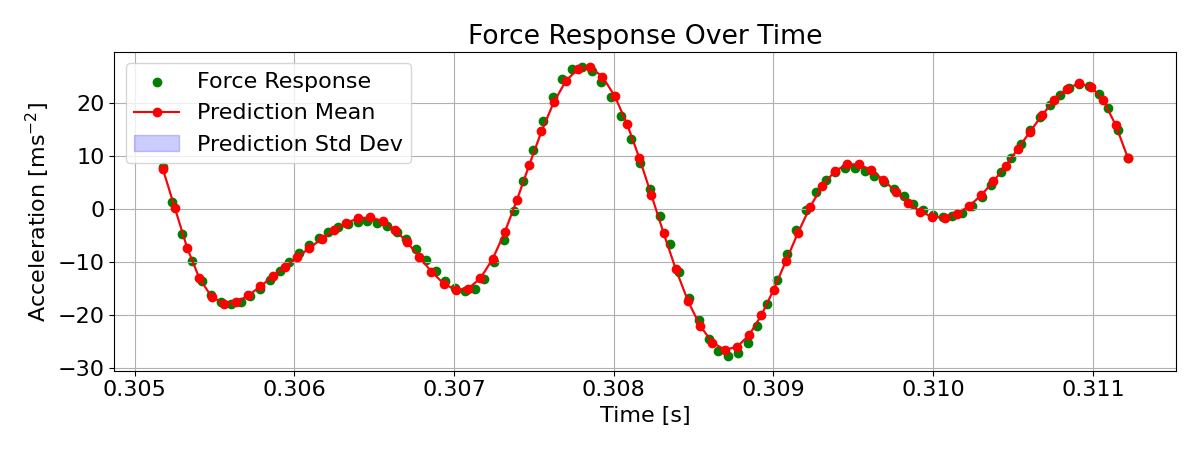
\includegraphics[width=1.0\linewidth]{figures/input-response-plot/input-response-plot.png}
        \caption{The time series data which the GP was fit to.}
        \label{fig:input-response-plot}
    \end{figure}



    \subsection{The Kernel}
    Next, a python class was created to contain the kernel.
    This is a special function that when input with two arrays, produces a covariance matrix that measure the similarity between each pair of inputs.
    The function is chosen to reflect any prior knowledge about the problem domain, and must ensure that the resulting matrix is symmetrical about the main diagonal, and have a property called Positive Semi-definiteness.
    To begin with, a white noise kernel (equation~\ref{eq:white-noise-kernel}) was chosen for the force input plot because there was no trend to the force input data in the centre of the time series data (seconds after the initial impulse from the impact from the hammer).
    This kernel ensures that ``all covariances between samples are zero because the noise is uncorrelated``~\cite{RoelantsGPKernels}

    \begin{equation}
        K_{ij} =
        \begin{cases}
            \sigma^2 & \text{if } \mathbf{x}_i = \mathbf{x}_j \\
            0 & \text{otherwise}
        \end{cases}\label{eq:white-noise-kernel}
    \end{equation}

    For the force response plot, a periodic kernel was chosen (Equation~\ref{eq:periodic-kernel}), which is ideal for such periodic data since it gives pairs of points a high similarity score if the difference between them is near an integer multiple of the `period` hyperparameter.
    The `length` hyperparameter determines how quickly this similarity drops off as the difference between the pair of points changes.
    Practically, this controls how smooth vs how wiggly the function is.

    \begin{equation}
        k(x, x') = \sigma^2 \exp\left(- \frac{2 \sin^2\left(\frac{\pi}{p} |x - x'|\right)}{l^2}\right)\label{eq:periodic-kernel}
    \end{equation}

    \subsection{Hyperparameter Optimisation}
    Next, this kernel class was added as an attribute to a class for the GP model itself.
    This allowed the kernel to be computed for different pairs of arrays as needed.
    This GP model also contained a method to optimise the hyperparameters of the kernel by minimising the Negative Log Marginal Likelihood.
    The algorithm did this by multiplying each hyperparameter in turn by the exponent of a normally distributed continuous random variable.
    If the new NLML was lower than the previous, the hyperparameter was updated.
    However, it also has a mechanism to help the algorithm from getting stuck in local minima.
    This is analogous to a ball rolling down a hill to towards the global minimum, if it always goes directly downhill, it may get stuck in a small valley before the lowest point, so it never optimises to find the global minimum, and should be avoided.
    The mechanism is as follows; if the new NLML was higher than the previous, the hyperparameter was maybe still updated at random, but with the probability of this occuring increasing as the new NLML became closer to the previous NLML\@.

    \subsection{Predict Function}
    Next, the predict function was constructed to predict the output to new inputs.
    This accurately predicted the mean and variance for locations between the training points, as shown in Figure~\ref{fig:input-response-predict}.
    The data is more noisy in the top Force Input than the Force Response plot, so the standard deviation is larger to take account for the noise.

    \begin{figure}[htbp]
        \centering
        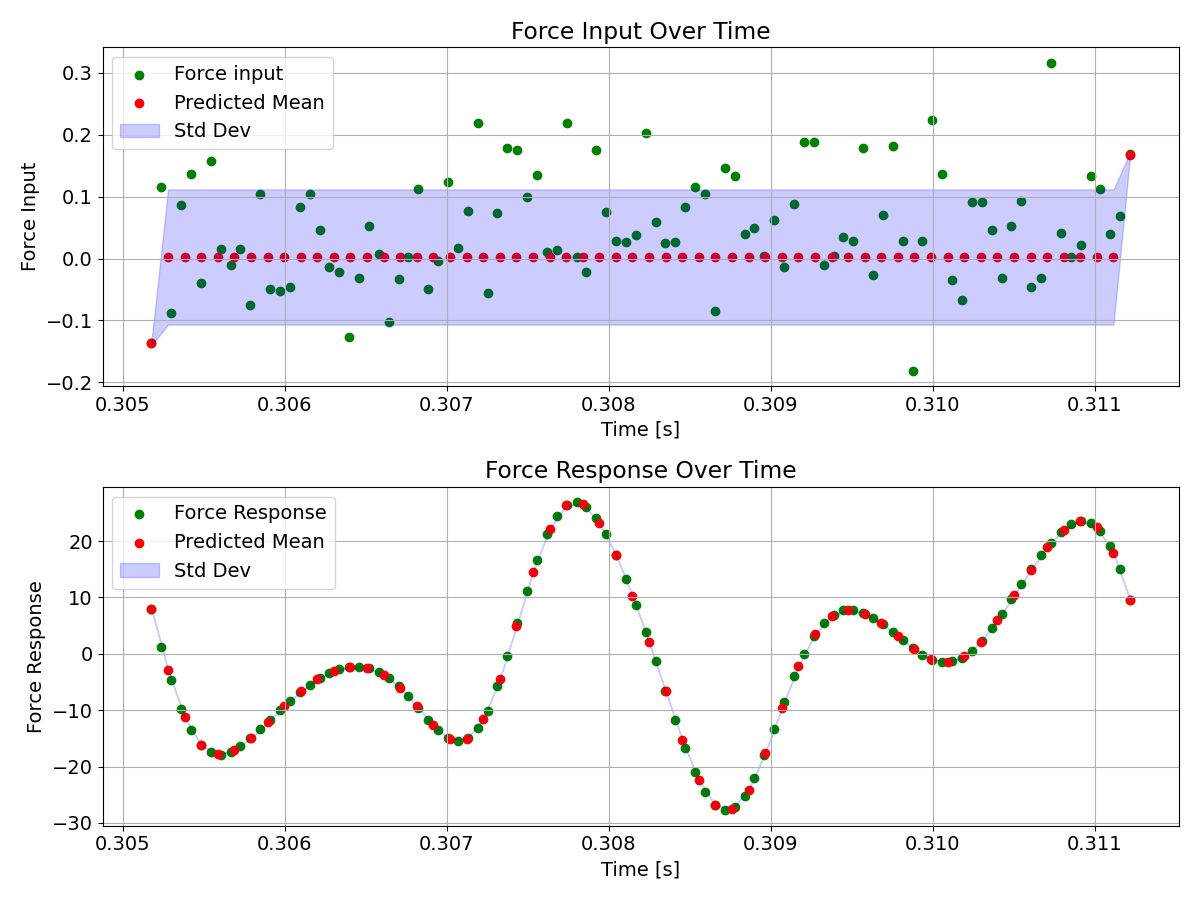
\includegraphics[width=1.0\linewidth]{figures/input-response-predict/input-response-predict.png}
        \caption{The prediction function fit by the GP overlayed on the training data. Note that the standard Deviation increases for data with more noise.}
        \label{fig:input-response-predict}
    \end{figure}

    \subsection{Sparse GP}
    Finally, the model modified to scale to large data, by converting it to a type of Sparse GP approximation known as FITC.
    This changed the $O()$ from $O(n^3)$ to $O(mn^2)$ for a set of m inducing points chosen to be a subset of the original training points, evenly spaced, where $n >> m$.
    This modification was made to the NLML and predict functions, which required a very specific implementation involving multiple mathematical tricks in order to keep the calculations numerically stable and efficient in terms of computation time and memory required
    This is because certain matrix operations such as determinants and inversions can give imprecise results for large matrices containing floating point numbers (a format that computes use to store continuous variables as a decimal, (as opposed to integers type variables)).
    After this was complete, the GP could be fit for functions containing more than 1000 data points with ease...

    \section{Plan for Future Work}
    After the Sparse GP, the next step will be to adjust the prediction function to be in a closed form so that the Fourier Transform can be taken.
    This means that the function will be defined symbolically so that it can be described in general instead of at a given set of input values.
    This can then be solved analytically/symbolically either by hand or using a Python package like SymPy, resulting in the Fourier Transform of the prediction function (i.e., the Fourier Transform of the discrete time series data) in closed form.

    The robustness to noise of the Fourier Transform of this model then needs to be compared to that of the standard discrete Fast Fourier Transform.
    To do this, the Frequency Response Function can be computed for both methods using the Fourier Transforms of the force input and responses.
    As a starting point, the Mean Squared Error (MSE) can be computed between the both, to see how different they are.
    The MSE is a method of measuring the quality of an estimator (lower is better) by measuring the average of the squares of the errors, as shown in Equation~\ref{eq:mse}

    \begin{equation}
        \text{MSE} = \frac{1}{n} \sum_{i=1}^{n} (Y_i - \hat{Y}_i)^2
        \label{eq:mse}
    \end{equation}


    Then, some Gaussian noise can be added to the data, and the FRF can again be computed using both methods again.
    To find how much each method is corrupted by noise, the (discrete) Mean Squared Error can be computed between the unmodified and noisy FRF for both Fourier Transform methods, and the values compared to find which method is more robust to noise.
    Note that for our new closed form Fourier Transform method, it would be possible to use a continuous method to compare the FRF with and without noise.
    An example of this is the L2 norm, which integrates the squared difference over a chosen domain, but this would have little utility because the same could not be calculated for the discrete FFT method for comparison.
    This analysis can be repeated for different amounts of noise, as well as different signals such as a pure sine wave, and finally a conclusion can be drawn regarding the utility of the new method presented in this paper.

    \subsection{Future Work Time Plan}
    Figure~\ref{fig:gantt-chart}a Gantt chart outlining the main steps and the approximate schedule for the remaining work in the project:

    \begin{landscape}
        \begin{figure}[p] % 'p' places the figure on a page of its own
            \centering
            \includegraphics[width=\linewidth]{figures/gantt_chart/gantt-chart_.png}
            \caption{A Gantt chart to show the time plan of the remaining work required to finish the project, using a format modified from~\cite{DataCampGanttChart2021}. For compactness, Tasks A - G are listed in the main body where this Figure is referenced.}
            \label{fig:gantt-chart}
        \end{figure}
    \end{landscape}





























































    \FloatBarrier
    \appendix
    \section{The use of generative AI (ChatGPT)}
    OpenAI's ChatGPT interface, powered by the GPT-4 large language model, was used to create some code.
    \subsection{\_inverse\_triangluar\_matrix\ method}
    This method is used to calculate the inverse of R in my method that computes the NLML in my FITC sparse GP approximation.
    It was generated using ChatGPT using the prompt: ``Write a Python function named \_inverse\_upper\_triangular that calculates the inverse of an upper triangular matrix in a faster and more numerically stable way than the standard np.linalg.inv function``.
    The output is provided in Figure~\ref{fig:chat-iut}.:
    \begin{figure}[htbp]
        \centering
        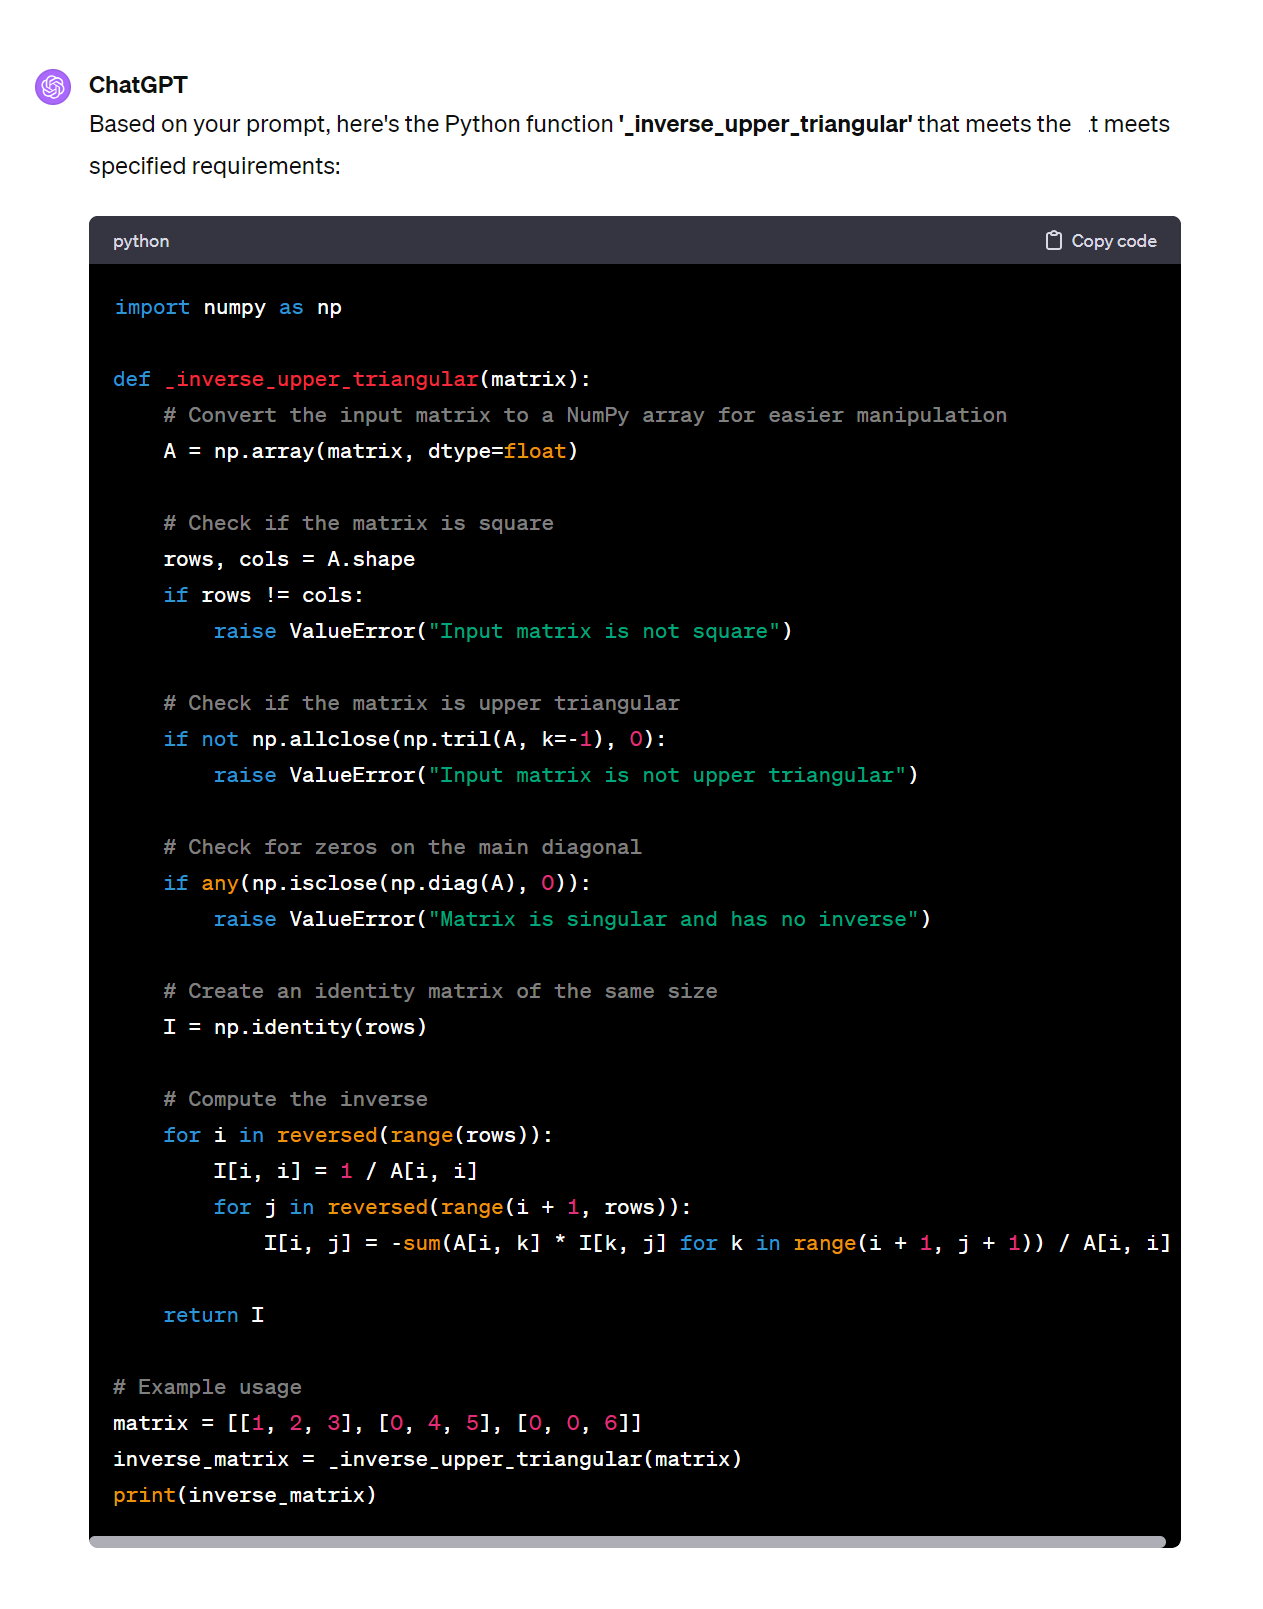
\includegraphics[width=0.8\linewidth]{figures/chat-iut/chat-iut.png}
        \caption{ChatGPT output providing a function used to inverse an upper triangular matrix in a faster and more numerically stable way}
        \label{fig:chat-iut}
    \end{figure}



    After this was generated, it was modified slightly to make it work in my FITC class.
    Firstly, it was made a method instead of a function by adding ``self`` to the inputs.
    Secondly, the output was transformed into a np.array type which is expected for the subsequent code.
    The resulting method is provided below:

    \FloatBarrier

    \begin{lstlisting}[language=Python]
    def _inverse_upper_triangular(self, matrix):
        # Convert the input matrix to a NumPy array for easier manipulation
        A = np.array(matrix, dtype=float)

        # Check if the matrix is square
        rows, cols = A.shape
        if rows != cols:
            raise ValueError("Input matrix is not square")

        # Check if the matrix is upper triangular
        if not np.allclose(np.tril(A, k=-1), 0):
            raise ValueError("Input matrix is not upper triangular")

        # Check for zeros on the main diagonal
        if any(np.isclose(np.diag(A), 0)):
            raise ValueError(
                "Matrix is singular and has no inverse")  # Changed from return None for consistency

        # Create an identity matrix of the same size
        I = np.identity(rows)

        # Compute the inverse
        for i in reversed(range(rows)):
            I[i, i] = 1 / A[i, i]
            for j in reversed(range(i + 1, rows)):
                I[i, j] = -sum(A[i, k] * I[k, j] for k in range(i + 1, j + 1)) / A[i, i]

        return np.array(I.tolist())
    \end{lstlisting}

    This was proven to work by writing a unit test:

    \FloatBarrier

    \begin{lstlisting}[language=Python]
    def test__inverse_upper_triangular(self):
        obj = GP_NLL_FITC(1, 2, 3, 4, 5, 6)

        # Upper triangular matrix
        matrix = np.array([
            [2, 3, 1],
            [0, 4, 5],
            [0, 0, 7]
        ])

        start_time = timer.time()

        result = obj._inverse_upper_triangular(matrix)

        end_time = timer.time()
        elapsed_time = end_time - start_time
        print(f"The _inverse_upper_triangular func ran in {elapsed_time} seconds")

        start_time = timer.time()

        correct = np.linalg.inv(matrix)

        end_time = timer.time()
        elapsed_time = end_time - start_time
        print(f"The np.linalg.inv func ran in {elapsed_time} seconds")

        debug_print(f"result = {result}")
        debug_print(f"correct = {correct}")
        debug_print(f"difference = {result - correct}")

        assert np.allclose(result, correct, atol=1E-5, rtol=1E-5)

        # Another upper triangular matrix with different values
        matrix2 = np.array([
            [-1.9883, 2.0, 3.0],
            [0, -9.4199, 4.0],
            [0, 0, 1.7969]
        ])
        start_time = timer.time()

        result2 = obj._inverse_upper_triangular(matrix2)

        end_time = timer.time()
        elapsed_time = end_time - start_time
        print(f"The _inverse_upper_triangular func ran in {elapsed_time} seconds")

        start_time = timer.time()

        correct2 = np.linalg.inv(matrix2)

        end_time = timer.time()
        elapsed_time = end_time - start_time
        print(f"The np.linalg.inv func ran in {elapsed_time} seconds")

        debug_print(f"result2 = {result2}")
        debug_print(f"correct2 = {correct2}")
        debug_print(f"difference2 = {result2 - correct2}")

        assert np.allclose(result2, correct2, atol=1E-5, rtol=1E-5)
    \end{lstlisting}


    This compared the result calculated by the method with an expected result calculated using the standard \texttt{np.linalg.inv} function for the two different input matrices.
    If they were the same within both a relative and absolute tolerance of $1E-5.$

    The unit test passed, showing that the function inverses the matrix correctly, however, it wasn't necessarily faster than the standard \texttt{np.linalg.inv} function.
    The inverse of the first matrix was calculated in $0.000246$ and $0.001368$ seconds using \texttt{\_inverse\_upper\_triangular} and \texttt{np.linalg.inv} methods respectively, whereas the inverse of the second matrix was calculated in $0.000312$ and $0.00005$ seconds respectively.
    This indicates that the fastest method depends on the input matrix, which is likely true for larger matrices also since both functions are of the $O(n^3)$ for an $n \times n$ matrix.
    However, the \texttt{\_inverse\_upper\_triangular} function will be more numerically stable and memory efficient because it is taking adavantages of the fact that the input matrix is upper triangular which allows the inverse to be found by back substitution instead of it being computed naively.
    \FloatBarrier

    \subsection{Figures for the report}
    \subsubsection{Cumulative Distribution Function}
    Put prompt and output


    \printbibliography

\end{document}
